%Ok, jag vet att vissa av dessa �r standard, men jag vill vara s�ker
\documentclass[a4paper,11pt,oneside]{memoir}

\usepackage[swedish]{babel}
\usepackage[T1]{fontenc}
\usepackage[latin1]{inputenc}

\usepackage{graphicx}
\usepackage{cite}
\usepackage{url}
\usepackage{listings}
\lstset{language=Java,numbers=left,frame=L,floatplacement=hbtp}
\def \lstlistingname {Kodexempel}


\pagestyle{plain}
\headstyles{komalike}
\nonzeroparskip
\setlength{\parindent}{0pt}
\checkandfixthelayout


\usepackage{ifpdf}
\ifpdf
	\usepackage[hidelinks]{hyperref}
\else
	\usepackage{url}
\fi

\usepackage{ifthen}

\newcommand{\assignmentNumber}[1]{\def \assignmentNumberValue {#1}}

\newcommand{\addressformatter}[1]{\ifthenelse{\equal{#1}{}}{}{(#1)}}

\newcommand{\authorOne}[4]{\def \authorOneLine {#1
#2 \addressformatter{#3}\\ \href{mailto:#4}{\nolinkurl{#4}}}}
\newcommand{\authorTwo}[3]{\def \authorTwoLine {#1 #2 \addressformatter{#3}\\}}
\newcommand{\authorThree}[3]{\def \authorThreeLine {#1 #2 \addressformatter{#3}\\}}


% D�ljer en varning
\author{}


\assignmentNumber{2}
\title{Projektets namn}

\authorOne{F�rnamn1}{Efternamn1}{anvnamn1}
\authorTwo{F�rnamn2}{Efternamn2}{anvnamn2}
\authorThree{}{}{}

\begin{document}

\frontmatter
\begin{titlingpage}


% Upper part of the page
\sffamily 

{\HUGE \bfseries Inl�mningsuppgift \assignmentNumberValue}\\
{\Large \thetitle}

\authorOneLine
\authorTwoLine
\authorThreeLine

\vfill



% Bottom of the page
{\LARGE Objektorienterad programmering}\\
{\tiny H�stterminen 2012\\
Kursansvarig: Henrik Bergstr�m}

\end{titlingpage}
\tableofcontents

\mainmatter

\chapter{Inledning}

Jag har byggt ett TicTacToe, �ven kallat tre-i-rad spel. Spelet g�r ut
p� att tv� spelare placerar pj�ser i ett nio rutors kvadratiskt rutn�t
best�nde tre rader och tre kolumner. Ett spel �r �ver n�r alla rutor
antingen n�r alla nio rutor har pj�ser eller n�r en enskild spelare
har plaserat sina pj�ser i alla rutorna i en vertikal linje,
horizontell linje eller en av de tv� av diagonalerna. Vinnaren �r den
spelaren som kontrollerar en av de ovann�mnda linjerna. Om ingen
vinnare kan koras s� anses spelet vara oavgjort.

\section{Akt�rer}
Spelet inkluderar tre stycken datorstyrda akt�rer, samt en som styrs
via ett textgr�nssnitt. 

\paragraph{RandomAI} Valet av ruta att placera pj�sen i helt �r helt
(pseudo-)slumpm�ssigt. Denna akt�r �r anv�ndbar f�r att testa andra
akt�rer.

\paragraph{FeedForwardNNAI} Denna akt�r anv�nder ett
Feed-Forward neuralt n�tverk best�nde av nio neuron i input lagret,
tre i det g�mda lagret, samt nio i output lagret. Denna akt�r
presterar helt klart b�ttre �n slumpen men spelar inte lika bra som en
typisk person. Det �r dock v�rt att n�mna att en m�nniska har ungef�r
85 miljarder neuron j�mf�rt med de arton neuron som anv�nds av mitt
program.

\paragraph{AlgoAI} Denna akt�r implementerar p� ett rent algoritmiskt
s�tt. Den till�mpar ett antal regler. I f�rsta hand f�rs�ker den hitta
ett l�ge d�r den kan placera en pj�s f�r att f� tre-i-rad, allts� att
vinna. I andra hand f�rs�ker den att blockera motst�ndaren fr�n att
l�gga tre pj�ser i rad. Den tredje regeln i prioriterings ordningen �r
att f�rs�ka skapa ett l�ge d�r spelaren f�r tv� m�jligheter till att
vinna n�sta tur. Ett exempel p� detta �r ett l�ge d�r man h�ller det
�vre v�nstra, �vre h�gra, samt nedre h�gra h�rnet. D� motst�ndare inte
kan blockera tv� m�jligheter p� en tur s� har man d�rmed vunnit. Om
ingen s�dan m�jlighet finns s� f�rs�ker vi blockera motst�ndarens
m�jligheter att utf�ra detta. Om inget av detta �r m�jligt placerar vi
i f�rsta hand mitten, d�refter h�rnen, och om detta ej �r m�jligt,
sidorna.

\chapter{Design}

H�r ska ni beskriva designen av systemet. Ett l�mpligt format �r ett klassdiagram kompletterat med en kort textuell beskrivning. Var noga med att redovisa vilka delar ni har gjort sj�lva och vilka som �r tagna fr�n Java eller fr�n andra bibliotek. F�r ett vanligt projekt b�r 2 sidor r�cka mer �n v�l f�r denna del. Har man en avancerad design 
\chapter{Kravuppfyllnad}

Nedan f�ljer de krav som skrevs i uppgiften, men �ven ett stycke om
testning.

\section{Samverkande klasser}
Klaserna i projektet samverkar i h�gsta grad. En akt�r (Actor)
kontrollerar en spelare (Player). En spelare deltar i ett spel (Game)
som spelas i ett rutn�t (Grid). Rutn�tet anv�nder rutor (Square) f�r
att h�lla kolla p� vem som har placerat pj�ser var. Rutn�tet
innefattar ocks� Linjer (Line) som anv�nds f�r att h�lla koll p�
vertikala, horizontella, linjer.

\section{Arv och polymorfism}
Arv och polymorfism anv�nds f�r att implementera olika sorters
akt�rer. Samtliga akt�rer �r subklasser av den abstrakta klassen Actor
som specificerar en method som kallas p� av Player. De olika
subklasserna har olika betenden f�r hur de ska spela.
\lstinputlisting{RandomAIEx.java}

\section{Namngivning}
Javas namngivnings regler har f�ljts till fullo, packet �r under en
dom�n som kontrolleras av mig, vilket hindrar namnkollisioner.
Variabler och methoder �r i \emph{lowerCamelCase}, med f�rkortningar i
versaler. Klasser i \emph{UpperCamelCase}, �ven h�r med f�rkortningar i
versaler. Jag har �ven f�rs�kt att undvika namn som best�r av flera
ord d� dessa kan tyda p� d�ligt genomt�nkt design eller bristande
terminologi.

\section{Korrekta skyddsniv�er}

Det finns inga publika f�lt i projektet utan samtliga getter metoder
anv�nds f�r att l�sa av v�rden. Detta g�mmer de under liggande
variablerna vilket leder till att det �r enkelt att �ndra p� hur den
underliggande f�rvaringen g�r till. Nedan f�ljer ett f�renklat exempel
av Square klassen.

\lstinputlisting{SquareSimp.java}

\section{Testning}

Programets delar testas av ett femtiotal Unit-test som anv�nds f�r att
verifiera programets funktionalitet. Dessa testa erbjuder inte
fullst�ndig t�ckning av koden, det saknas helt tester f�r akt�rerna
och gr�nssnitt. D�remot s� �r t�ckningen n�stan fullst�ndig f�r koden som
implementerar dom�nmodellen.

\par JUnit4 tillsamans med Apache Maven anv�nds f�r testerna. Maven
kommandot \texttt{mvn test} kan anv�ndas f�r att k�ra samtliga test.



\chapter{Reflektion}

Den sista delen i rapporten �r t�nkt f�r egenreflektion. Vad har fungerat bra? Vad har fungerat d�ligt? Var uppgiften f�r l�tt? F�r sv�r? �r det n�got ni borde ha �vat mer p� innan ni satte ig�ng? �r det n�got vi borde ha �gnat mer tid �t eftersom ni beh�vde det?

\chapter{Mallanv�ndningen}

Detta avsnitt tar upp n�gra vanliga fr�gor/problem med mallandv�ndningen. Det ska naturligtvis plockas bort i den version ni l�mnar in.

\section{Bilder}

Bilder ska tillf�ra n�got till texten, vara tydliga, ha en f�rklarande bildtext, och sitta p� ett vettigt st�lle i f�rh�llande till texten. De b�r ocks� refereras till i texten. T�nk p� att bilder i \LaTeX{} b�r placeras i floats, och att dessa kan flyttas runt automatiskt. Du m�ste allts� anta att bilden kan flyttas runt om du g�r n�gra �ndringar. Man b�r allts� alltid referera till figurer med hj�lp av labels: Figur \ref{fig:Exempelbild} p� sidan \pageref{fig:Exempelbild}.

\begin{figure}[htbp]
	
	\begin{center}
	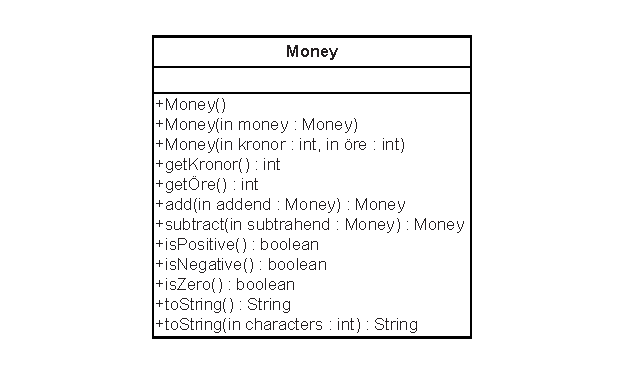
\includegraphics{money}
	\end{center}
	
	\caption{Exempelbild}
	\label{fig:Exempelbild}
\end{figure}

\subsection{Rubrikniv� 3}

Rubrikniv� tre och ner�t b�r man normalt undvika att anv�nda. Ibland g�r det inte, men ofta �r det ett tecken p� att man delar upp sitt dokument i f�r sm� bitar.

\section{Referenser}

Referenshanteringssystemet till \LaTeX{} heter BibTex, och det ska man naturligtvis anv�nda. P� OOP anv�nder vi IEEE:s format med numrerade referenser inom hakparanteser. En referens till kursanvisningarna skulle allts� se ut s� h�r: \cite{OOP}, eller s� h�r om man vill ha med sidanvisningar: \cite[s.~5]{OOP}.

\section{Kod}

Kod i dokumentet ska naturligtvis vara l�sbar och helst formaterad som i en utvecklingsmilj�. Ett tips �r att inte anv�nda sk�rmdumpar. De blir n�stan alltid ol�sliga, och det g�r inte att f� ut k�llkoden fr�n dem om man skulle vilja.

Mallen anv�nder sig av listingspaketet (\url{http://mirror.hmc.edu/ctan/macros/latex/contrib/listings/listings.pdf}) som kan formatera kod antingen direkt i latexkoden som i exempel \ref{lst}, eller fr�n en fil som i exempel \ref{lst:fil}. Man kan �ven plocka ut vissa rader ur en fil som i exempel \ref{lst:filrader}.

Inst�llningarna f�r programspr�k, radnumrering, etc.\ finns i direkt anslutning till d�r paketet importeras i latexmall.tex.

\begin{lstlisting}[float,caption={Kod som ligger i latexfilen},label=lst]
class Exempel{

	int number;

}
\end{lstlisting}

\lstinputlisting[float,caption={Kod som h�mtas fr�n fil},label=lst:fil]{Exempel.java}

\lstinputlisting[float,firstline=3,lastline=3,caption={En rad fr�n en fil},label=lst:filrader]{Exempel.java}

\section{Avsnitt i mallen}

Den text som finns i mallen �r naturligtvis avsedd bara f�r att illustrera anv�ndningen. Har ni, till exempel, inte n�gra bilagor plockar ni naturligtvis bort dessa fr�n dokumentet.




\bibliographystyle{plain}
\bibliography{bibtex}
\bibdata{bibtex}

\appendix
% \chapter{Bilagsrubrik}


\end{document}
